\documentclass[a4paper,10pt]{article}

\usepackage{préambule}

\TitreDActivite{Activité : Proportionnalité}

\begin{document}

\maketitle

\section{Construction et mesure}
\begin{enumerate}
	\item Place deux points A et B.
	\item En utilisant l'outil \squared{Cercle(centre,point)}, construis un cercle c de centre A et passant par B.
	\item Trace le segment [AB].
	\item Puis, utilise l'outil \squared{Distance ou longueur} pour afficher les longueurs suivantes :
	      \begin{enumerate}
		      \item La longueur AB.
		      \item Le périmètre du cercle c.
	      \end{enumerate}
\end{enumerate}


\section{Tableur}
Ouvre un tableur dans Geogebra, en sélectionnant \squared{Affichage $→$ Tableur} dans le menu.

Reproduis le tableau de la figure ci-dessous :

\begin{center}
	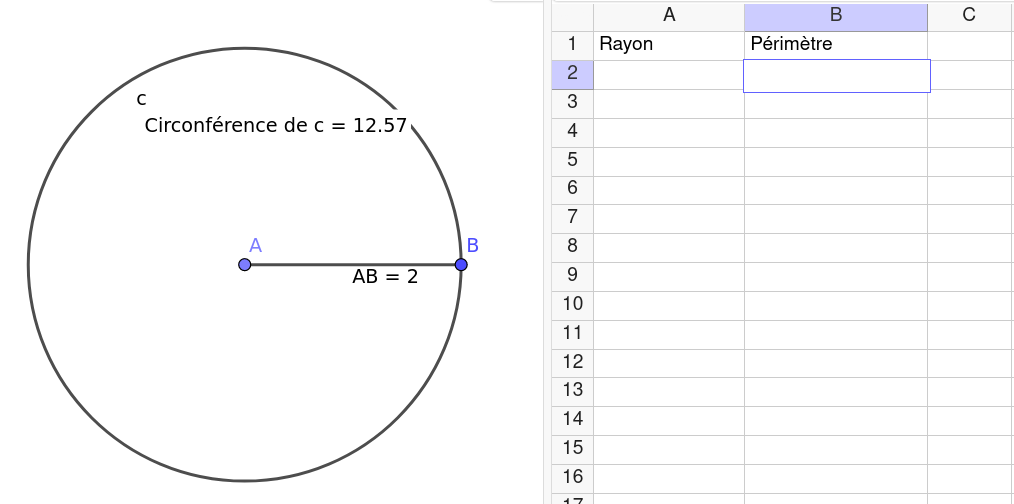
\includegraphics[width=0.7\linewidth]{Images/Geogebra - figure pi.png}
\end{center}

\begin{enumerate}
	\item Dans la deuxième ligne, note le rayon et le périmètre de ta figure.
	\item Déplace le point B pour que la longueur de AB soit 4. Note dans la troisième ligne le nouveau rayon et périmètre.
	\item Procède ainsi pour des rayons de longueur 8, puis 12, jusqu'à remplir la ligne 5.
	\item Le rayon et le périmètre semblent-ils proportionnels ? Que faudrait-il faire pour le vérifier ?
\end{enumerate}

\section{Proportionnalité}
Pour étudier un peu plus cette question, nous allons calculer le rapport entre le périmètre d'un cercle et son rayon.

\begin{enumerate}
	\item Dans la case C2, écrit une formule qui permet de calculer
	      $$ \text{périmètre} ÷ \text{rayon} $$
	\item Étens cette formule pour les autres cercles que tu as construis. Que remarque-t-on ?
	\item Émet une conjecture sur la valeur du coefficient de proportionnalité.
\end{enumerate}

\section{Valeur exacte}

\begin{enumerate}
	\item Crée un nouveau cercle de rayon 0,5 (avec l'outil \squared{Cercle(centre-rayon)}), et affiche son périmètre. Quel est ce périmètre ? ..........
	\item En déduire la valeur du coefficient de proportionnalité .............
	\item Retrouver la formule du périmètre P d'un cercle de rayon r.
\end{enumerate}

\awesomebox[violet]{2pt}{\faRocket}{violet}{
	\textbf{Pour aller plus loin}

	Construis un cercle de périmètre 20, et explique ta démarche.
}


\end{document}